%%%%%%%%%%%%%%%%%%%%%%%%%%%%%%%%%%%%%%%%%%%%%%%%%%%%%%%%%%%%%%%%%%%%
% Grundlagen
%%%%%%%%%%%%%%%%%%%%%%%%%%%%%%%%%%%%%%%%%%%%%%%%%%%%%%%%%%%%%%%%%%%%

\chapter{Material and Methods}
  \label{MetMat}

\section{Data}
  \label{Data} 
  
\subsection{Data acquisition}
  \label{DataAcq}

The original Dataset consists of 947 whole slide images from 176 Patients. The patients were treated at the Hannover Medical School (MHH) hospital between 1992 and 2022. Most images have region-level annotations associated to them that define the tissue and the tumour areas at different levels of granularity.
For a subcohort of 24 patients, expression counts of cancer-relevant genes are also available. These were acquired using the NanoString panel nCounter\textsuperscript{\textregistered} PanCancer IO 360\texttrademark. This assay comprises 770 genes that are categorised into 16 categories, each belonging to either one of the groups 'Tumor', 'Microenvironment' or 'Immune Response'. A subset of 20 genes makes up an internal reference. \cite{NanoStringTechnologies2017Gene}
Figure \ref{fig:SurvStats} visualises both the subcohort with their respective survival times and the overall distribution of patients  with respect to their survival times.

\begin{figure}[htb]
    \centering
 \begin{subfigure}[b]{0.59\textwidth}
 \centering
    \includegraphics[width=\textwidth]{latex/figures/survival_days_distribution_hires_evenly_binned.png}
     \caption{Distribution of survival times}
     \label{fig:SurvHisto}
 \end{subfigure}
    \hfill
 \begin{subfigure}[b]{0.4\textwidth}
 \centering
     \includegraphics[width=\textwidth]{latex/figures/surv_race_rcc.png}
     \caption{Survival time of subcohort}
     \label{fig:SurvRaceSmall}
 \end{subfigure}
  \caption[Cohort visualisation]{Distribution of survival times and concrete survival times of patients with gene expression data. An extension of \ref{fig:SurvRaceSmall} for the full cohort can be found in the appendix \ref{fig:SurvRaceFull}}
  \label{fig:SurvStats}
\end{figure}


\subsection{Pyramidal Images as SVS files}

The image files are provided as ScanScope Virtual Slides (SVS) files. This is the file format used by Aperio scanners for glass microscope slides. They represent a modification of regular TIFF files, such as altered tag structure and additional metadata. These files also use JPEG2000 or JPEG. This makes it feasible to store them in files smaller than 4 gigabytes. This is necessary as the underlying TIFF file format only supports file sizes below that threshold. \cite{AperioTechnologies2008Digital} TIFF files can hold multiple images with different sizes. Therefore, it is possible to bundle the same image at different resolutions within the same file. \cite{Aldus1992TIFF} 
This can practice can commonly be found in pathology image to represent different downsampling scales of the same slide image. Figure \ref{fig:pyramid}
However, due to the complexity of the file format, there are multiple possible ways to internally represent an image hierarchy in such files. \cite{Aldus1992TIFF} 
For example, the lower resolution files can be stored as extra 'pages' or as 'subfiles'.
This, in turn, limits the interoperability of different TIFF-based file formats used for digital pathology. It also increases the development burden on the applications and tools dealing with these files. The same problems occur for the metadata provided with each file, for example, SVS files use the TIFF metadata-tag “ImageDescription” to store information as key-value pairs. \cite{AperioTechnologies2008Digital} Meanwhile, the competing “OME-TIFF” format manages to store the meta-information formatted as XML within that tag. \cite{OpenMicroscopyEnvironment2022OME} 

\begin{figure}[h!t]
    \centering
    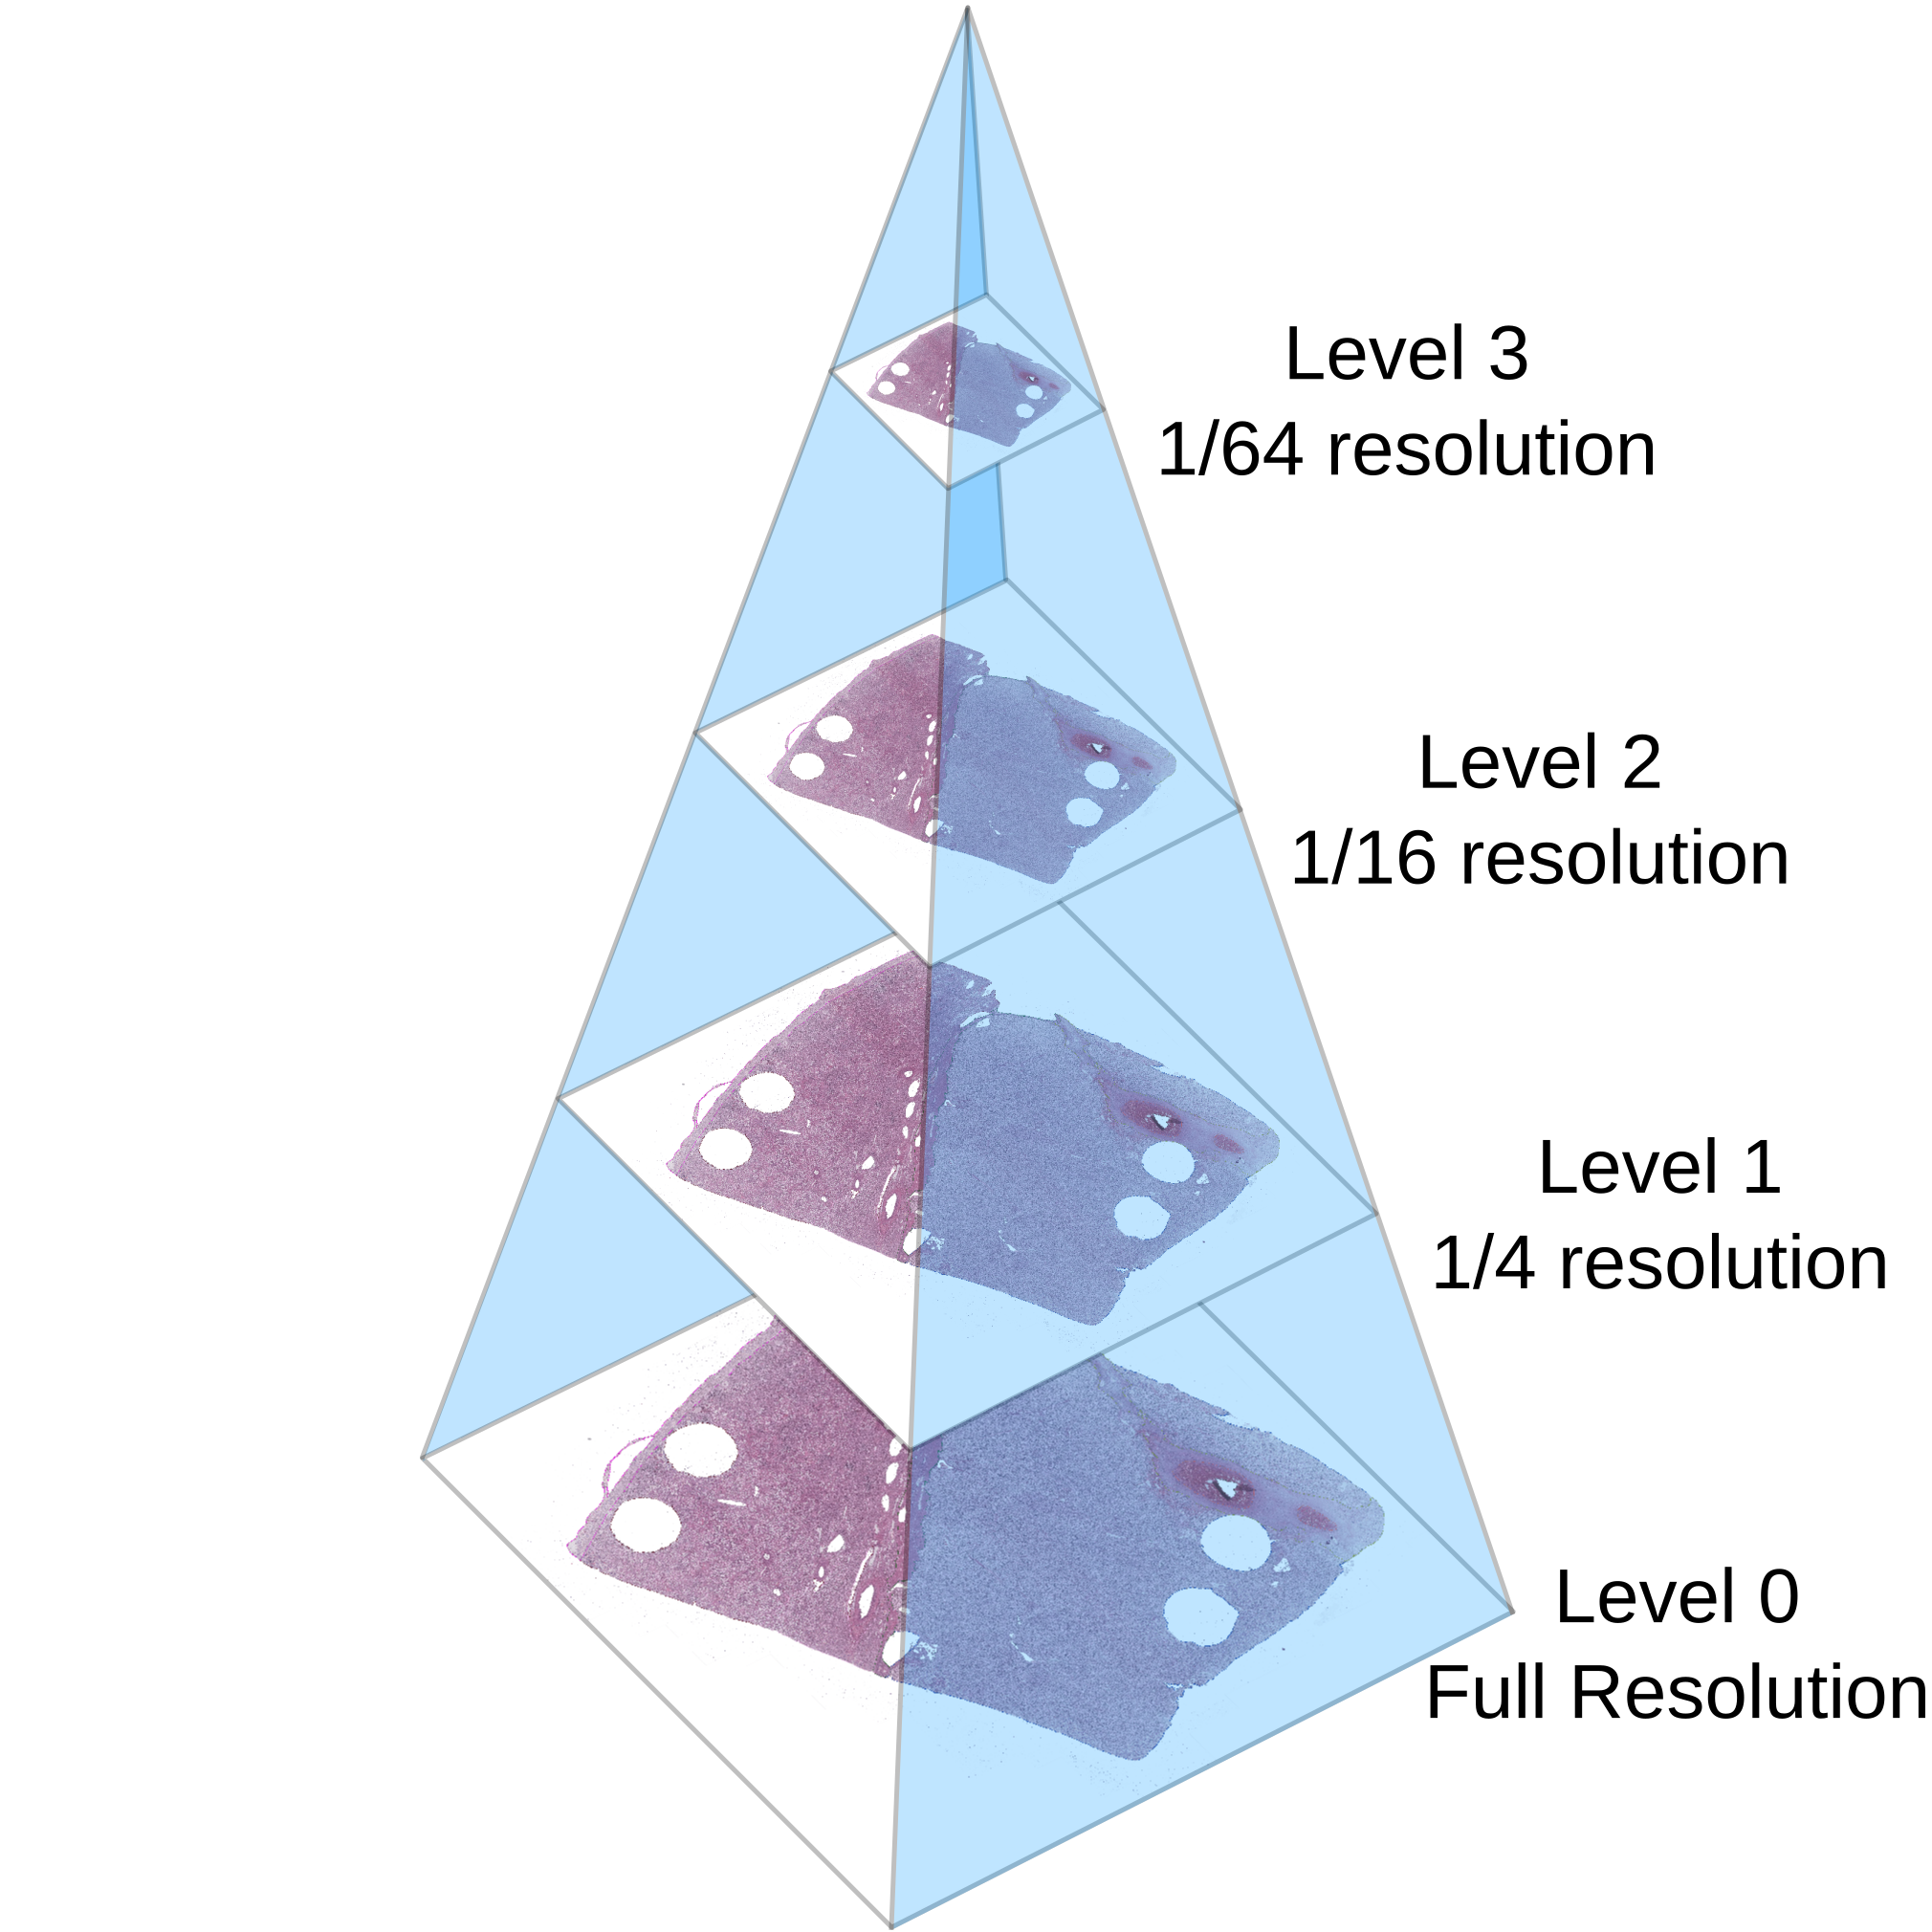
\includegraphics[width=0.6\textwidth]{latex/figures/Image_pyramid_centered.png}
    \caption[Pyramid representation of TIFF files]{Pyramid illustration of SVS files. The SVS format downsamples images by a factor to the power of four and saves them as separate pages. The page at index 0 contains the full resolution image, index 1 contains a special thumbnail. The following indices are used for the downsampled versions. Adapted from 'Illustration of an image pyramid with 5 levels.' by Cmglee (CC BY-SA 3.0). \cite{CreativeCommons2007Attribution, Cmglee2015Illustration} The figure was modified using Inkscape (version 1.2.2), a free and open source vector graphics editor. \cite{InkscapeTeam2022Inkscape}}
    \label{fig:pyramid}
\end{figure}

\subsection{Annotations and the GeoJSON file format}

The WSIs were annotated using the software QuPath, which was created for dealing with pathology images. \cite{Bankhead2017QuPath} Because of that, the annotations are not easily accessible and first have to be extracted from the respective QuPath projects. 
The python library \verb|paquo| was used to extract these individual annotations and export them as GeoJSON files. As the name suggests, the GeoJSON file format was originally invented to deal with high-resolution satellite images. \cite{Butler2016GeoJSON} Coincidentally, digital pathology images have a similar need for a lightweight, easy-to-parse file format to carry spatial information. The name also suggests that this is derived from the JSON file format. In fact, these files are valid JSON documents with pre-defined structures and names for keys and values. These files consist of an array of region objects and are made up of one or multiple arrays of coordinates that define one region's outline. In addition, each array is associated with various metadata; the individual keys are defined by either QuPath or the GeoJSON specification. \cite{Butler2016GeoJSON, Bankhead2017QuPath}. Only a subset of available annotations is used for this thesis. Those are the ones deemed most relevant to the task of the DNN. Concretely, the annotations are “Angioinvasion”, “Tissue”, “Tumor necrosis”, “Tumor regression” and “Tumor vital”. Figure \ref{fig:downsample_overlaid} shows a few examples of WSI with those annotations overlaid in the specified order. The medical interpretation is self-explanatory for most annotations. As Angioinvasion is the spread of tumour into a blood vessel, these annotations are generally much smaller in area and also rarer to occur than the regular tumour annotations.

\begin{figure}[h!t]
    \centering
    \includegraphics[width=0.32\textwidth]{latex/tissue/postproc_subimage_90-19_noLabel.png}
    \includegraphics[width=0.32\textwidth]{latex/tissue/postproc_subimage_109-42.png}
    \includegraphics[width=0.32\textwidth]{latex/tissue/postproc_subimage_19-42_noLabel.png}
    \caption[WSI and overlaid masks]{Tissue slides with annotations overlaid. The tissue annotation is only visible in areas without other annotations. It can be assumed that any non-white area of the image is marked as tissue. All images are taken at the same scale.}
    \label{fig:downsample_overlaid}
\end{figure}

\subsection{Data quality}

Multiple samples had to be removed from the dataset for reasons stemming from various issues with the data.

\subsubsection{Patient filtering} 
Data from whole patients had to be removed for two reasons. For once, this included patients who were affected by a cancer subtype other than the most prevalent one. Thus, only patients who were affected by clear cell renal Cell Carcinoma (RCC) were considered in this work. That is, because the morphological differences with other subtypes are too large and their subcohorts are too small in sample size to foster significant learning. This aspect reduced the number of patients from 176 to 141. 
In addition, not all the images provided were part of the study. Some images did not belong to the cohort of RCC patients at all, and others lacked any occurrence in one of the provided QuPath projects. Images of Patients that do not occur in any QuPath project also do not have any annotations. 
The second reason for removing patients is more pragmatic. In those cases, the necessary data for performing survival analysis is missing. For example, the time of the nephrectomy, which was used as the starting time, was missing.

\subsubsection{Image filtering} 
Next is the quality of the annotations. Since they are used for tissue segmentation, it is critical that they are present and usable. There are three reasons why patients were excluded from the analysis based on tissue-level annotations. First, 4 of the extracted GeoJSON files were empty. Most probably, because the image did not get properly annotated in the first place. Next, there were cases where only the tissue annotation is missing. This occurrence manifested in two forms. In the first case, the whole tissue-related entry in the GeoJSON file is missing, which happened in another 4 cases. However, some files do carry odd annotations that were only missing a classification. Whether that (or which, in the case of multiples per file) is the tissue-level one is difficult to determine without manual inspection by a domain expert. Therefore, these 13 images were also excluded.
The complete data provided consisted of 947 images and 176 patients. In the end, 705 images remained, out of which 495 belonged to the uncensored patients. The MHH provided up to five WSIs of different stains, consisting of one H\&E stain and four images stained with immunohistochemistry (IHC) staining. However, as explained above, not all patients had five usable images. 
This affected the balance of the resulting data sets at the slide level, in the sense that some patients contributed one or two fewer images to the data set. That being said, with only 21 images or 2.9\% removed, we concluded that this slight imbalance is negligible. 

\subsubsection{Data Quality and Edge cases}
There are still a few issues with the quality of the data samples that passed the preliminary filtering. This results in multiple edge cases that need to be handled during preprocessing of images and tile extraction. First, some images contain annotations that go beyond the boundaries of the image itself. Hence, these have to be identified, and their annotations have to be adjusted to the true image borders. We achieve this fast and efficiently by using the GeoJSON annotation files and the metadata stored inside the respective SVS files. Figure \ref{fig:OOB} illustrates this problem. Here, the annotation is not only outside the tissue area but also outside the image itself. In the annotation files, this is indicated by negative coordinate values.  As a solution, we simply set these coordinates to zero or to the width and height of the image, to restrain the annotations to stay within the bitmap.
Also, the tissue annotations often do not truthfully cover the area they are supposed to. 
Figure \ref{fig:CutOff} shows how annotations do not perfectly align with the WSI they correspond to. This does not only occur at the image boundaries, but over the whole border of the tissue. These issues become more prevalent due to the fact that our approach relies on the quality of these annotations heavily and trusts them blindly. There is a chance that these issues affect the performance of the model.
Furthermore, in a few samples the picture does not cover the whole tissue, the slide is cut off at one end of the image. There is nothing that can be done about these cases. Examples of these issues are shown in Figure \ref{fig:shitshow}.
Figure \ref{fig:ScanningIssue} illustrates the impact a contaminated slide can have on the scan quality. Normally, the scanned image is automatically cropped to the tissue's dimensions. However, if the scanner does not properly detect a distant tile to be empty, it will not cut off the space in-between. These misclassified TIFF tiles lead to wasted disk space and requires preprocessing of images, as described in \ref{DownsampleData}.


\begin{figure}[h!t]
    \begin{subfigure}[b]{0.62\textwidth}
      \includegraphics[width=\textwidth]{latex/QuPathScreenshots/shitty_scan_cropped.png}
      \caption{Erroneous WSI Scan}
      \label{fig:ScanningIssue}
    \end{subfigure}
    \hfill  % NOTE1: hfill moves horizontally stacked objects as far apart as it can
    \begin{subfigure}[b]{0.36\textwidth}
      \begin{subfigure}[t]{\textwidth}
        \includegraphics[width=\textwidth]{latex/QuPathScreenshots/annotationTooSoonSmall.png}
        \caption{Annotation cuts off tissue}
        \label{fig:CutOff}
        \vspace*{5mm}
      \end{subfigure}
    \\
      \begin{subfigure}[b]{\textwidth}
        \includegraphics[width=\textwidth]{latex/QuPathScreenshots/AnnotationOutsideSmall.png}
        \caption{Annotation out of bounds}
        \label{fig:OOB}
      \end{subfigure}
    \end{subfigure}
    \caption[Whole slide image quality]{Quality issues of Whole slide images (WSI). Multiple quality concerns with image data and their annotations are shown. Figure \ref{fig:ScanningIssue} demonstrates a failure of the scanning optimisations done by the WSI scanner. Figure \ref{fig:CutOff} shows an annotation border (recoloured in green for visibility) that removes image data from the tissue area. Figure \ref{fig:OOB} shows an annotation that reaches outside the image boundaries. The area outside the bitmap is shown in green.}
    \label{fig:shitshow}
  \end{figure}

Another problem worth noting is the amount of available resolutions. Either 3 or 4 lower-resolution images were embedded into each SVS file. These inconsistencies made the lowest resolution difficult to use. It would still be non-ideal to manually downsample the subset of images, where level 4 images are missing. Since we do not know the concrete algorithm and parameters used for downsampling, it is hard to reproduce fully compatible images. Hence, this would introduce a bias in the data.
Also, problematic is the treatment of file names. Although, there was an attempt to label each file in a structured manner, this has not been upheld properly for the entire data set. Especially for files that  seemed to be retaken, a suffix (e.g. 'flipped') was added either to the new or the old file. Since a suitable delimiter was missing, this made parsing case ID and stain code difficult. The quickest solution was to employ regular expression based string matching to capture the desired information more easily. This worked well for our dataset, but will require adjustment if new data is added.

\subsection{NanoString data and RCC files}

For a subset of 24 patients, a gene expression analysis was performed. The NanoString panel nCounter\textsuperscript{\textregistered} PanCancer IO 360\texttrademark provides information on 750 genes involved in the interactions between the tumour, the microenvironment, and the natural immune response. The detected genes are categorised by 48 biological signatures that are "potentially predictive Research Use Only". Data collection from biological samples was carried out \textit{via}two cartridges, each with 12 lanes for samples. \cite{NanoStringTechnologies2017Gene}

\subsubsection{Data Description}

Raw gene expression data is provided in the form of so-called RCC files, one per patient. In structure, these files resemble a list of XML tags, with each tag being pre-defined and containing relevant information. This means that, unlike sane XML formats, a root node is missing, or rather it is represented by the file itself. Hence, automated unmarshalling was not possible, and the file had to be scanned line-by-line for these XML-elements. The \verb|Code_Summary| tag contains the needed expression data in comma separated values (CSV) format. Each of these tables consists of one gene per row, where each row contains a category (\verb|CodeClass|), the name of the gene, its accession ID, and the corresponding raw count. The categories define whether the gene is a housekeeping gene, a positive, or negative control (both exogenous), or an endogenous gene of interest. 
Negative controls establish a background and the Limit of Detection (LOD), while positive controls are used to assess the quality of the assay. \cite{NanoStringTechnologies2017Gene}

\subsubsection{Quality Control}

First, a simple quality control (QC) was performed, which included multiple checks. The binding density represents the concentration of barcodes measured by the instrument per square micron. Separation of each probe from the others may not be possible if too many are present. If the density is too low, the results not meaningful. Therefore, samples with a binding density below 0.05 or greater than 2.25 must be removed. This upper limit is required for the case where barcodes overlap and thus impacts the quality of detection.  
The binding density is influenced by the target gene expression, RNA degradation, as well as the amounts of target genes and RNA loaded into the assay. \cite{NanoStringTechnologies2017Gene, Gorman2022IO}

The positive control linearity is a per-sample measure that assesses the quality of positive controls. It measures the linear increase of counts and relative concentration of the positive controls using the R\textsuperscript{2} metric of the concentration versus the raw counts. Positive controls are created by “spiking in” RNA into the samples in accordance to a linear dilution series. \cite{NanoStringTechnologies2017Gene, Gorman2022IO}

The Limit of Detection (LOD) confirms that the per-sample detection of positive controls is sufficiently above the one of the negative controls. It is calculated per sample, and the chosen threshold is calculated using the following symbolic formula:
\[ \textit{Average of negative controls} + 2 * SD \]
where \(SD\) stands for standard deviation. The second-lowest positive control, called \verb|POS\_E|, must have more raw counts than this baseline to pass this QC. The required information for this analysis was calculated based on the counts and extracted from the \verb|Lane_Attribtes| Tag. Fortunately, all 24 samples passed these checks.
Furthermore, the data is normalised first using the positive controls. Then the same is done with the included housekeeping genes. Each time, the mean of the respective gene subset is used to calculate a background and then subtracted it from the remaining data set. Neither the controls nor the housekeeping genes are later used as part of the input to the neural network.
Due to the reduced number of samples, the data is substituted by zero-filled arrays for patients for whom only image data is available. This is only for multimodal networks.
\cite{Gorman2022IO}

\subsubsection{Baseline Model}
For the gene expression data, a simple baseline model was trained before constructing the neural network. The Python package \verb|lifelines| was used to fit a traditional CPH model to genomic data. For this purpose, \(l_2\) regularization with a regularization rate of \(\lambda = 0.1\) was used.

\subsection{Mask generation}
\label{MakeMasks}

The python library \verb|rasterio| is used to rasterise GeoJSON files and convert them to arrays of dimensions equal to their corresponding WSI. This is preceded by parsing the GeoJSON file into \verb|Geometry| objects from the python library \verb|shapely| which serve as input into \verb|rasterio|. The extracted masks are then saved as pyramidal TIFF files following the BigTIFF specification. However, because these files adhere to common standards, they are downsampled using a different exponential factor. Therefore, masks are available at resolutions which are incrementally halved per level. The consequence of this is that more levels need to be stored in the file to contain the one corresponding to the WSI resolution of our approach. Fortunately, this does not cause significant storage overhead thanks to modern compression algorithms. Using the lossless algorithm \verb|zstandard| at compression level 3, each file, one per annotation per WSI, can be stored using only a small double-digit number (or less) of megabytes. For comparison, one SVS file takes at least 1.5 gigabyte to store, the worst offenders can take over 25 gigabytes of disk space.

\subsection{Patch Extraction}
  \label{PatchExtr}

A common approach to extract patches from whole slide images is to do so as part of preprocessing. Either, they are sampled from a grid and filtered afterwards \cite{Ren2018Recurrence, Cheerla2019Deep}  or extracted  based on a previously generated segmentation mask. \cite{Chen2021Whole, Chen2021Whole, Lu2021Data, Iizuka2020Deep}
Both require extra computation time and significant amounts of extra storage space. Another issue is the manner of patch extraction. When they are sampled from a grid, naturally, some of them will contain very little tissue content. Removal of these patches means a loss of potentially valuable information. The alternative, which is done sometimes, is to only sample patches randomly from the region of interest. Since this usually will not cover the whole area of the tissue, this approach loses potentially valuable information as well.
For survival analysis especially, we believe that it is ideal to maintain all input information. Because both benign and malignant tissue contribute towards the survival expectancy of individuals. For simple slide level classification, on the other hand, it is sufficient to use a subset of image patches. Under the condition that the selected ones are relevant, of course. For classification of objects within respective patches, it is even easier, as no global information is required.
This work presents an improved approach that manages to extract patches from a grid that is overlaid and adjusted to each individual WSI. There is no redundant utilisation of disk space and only optional and minimal preprocessing, while patch extraction still is reasonably efficient in terms of memory requirements and processing speed. We achieve this with the available annotations of tissue regions. However, even if that were not the case, tissue segmentation masks of similar or (unfortunately) better quality can easily be created using techniques such as otsu thresholding. \cite{Otsu1979Threshold} Furthermore, TIFF files allow regional read, which allows us to only load parts of an image at the same time to memory.

An annotation of tissue can be easily used to create a grid of coordinates for extraction of patches. Each of these points describes the top-left corner of the patch. Because of this, some of these coordinates lie, in fact, outside the tissue itself. This way, we properly capture all parts of the tissue, even at the edges. Furthermore, patches that would be empty (due to holes or tears within the tissue) are also excluded from extraction. This grid is aligned in horizontal bands over the tissue. This means that the patches at the left and top ends of the tissue are properly centred around the tissue region of the patch. Obviously, due to the grid being aligned gapless, this property cannot be ensured for the bottom or right end of the tissue. 
The implementation of this behaviour is performed using the \verb|shapely| package. With this package, GeoJSON annotations can easily be converted into \verb|Geometry| objects, and then queried for the annotations' edges or with specific coordinates. This is then used to align and generate bands of patches, as well as filter them according to the previously established rules. 

\begin{figure}[h!t]
    \centering
    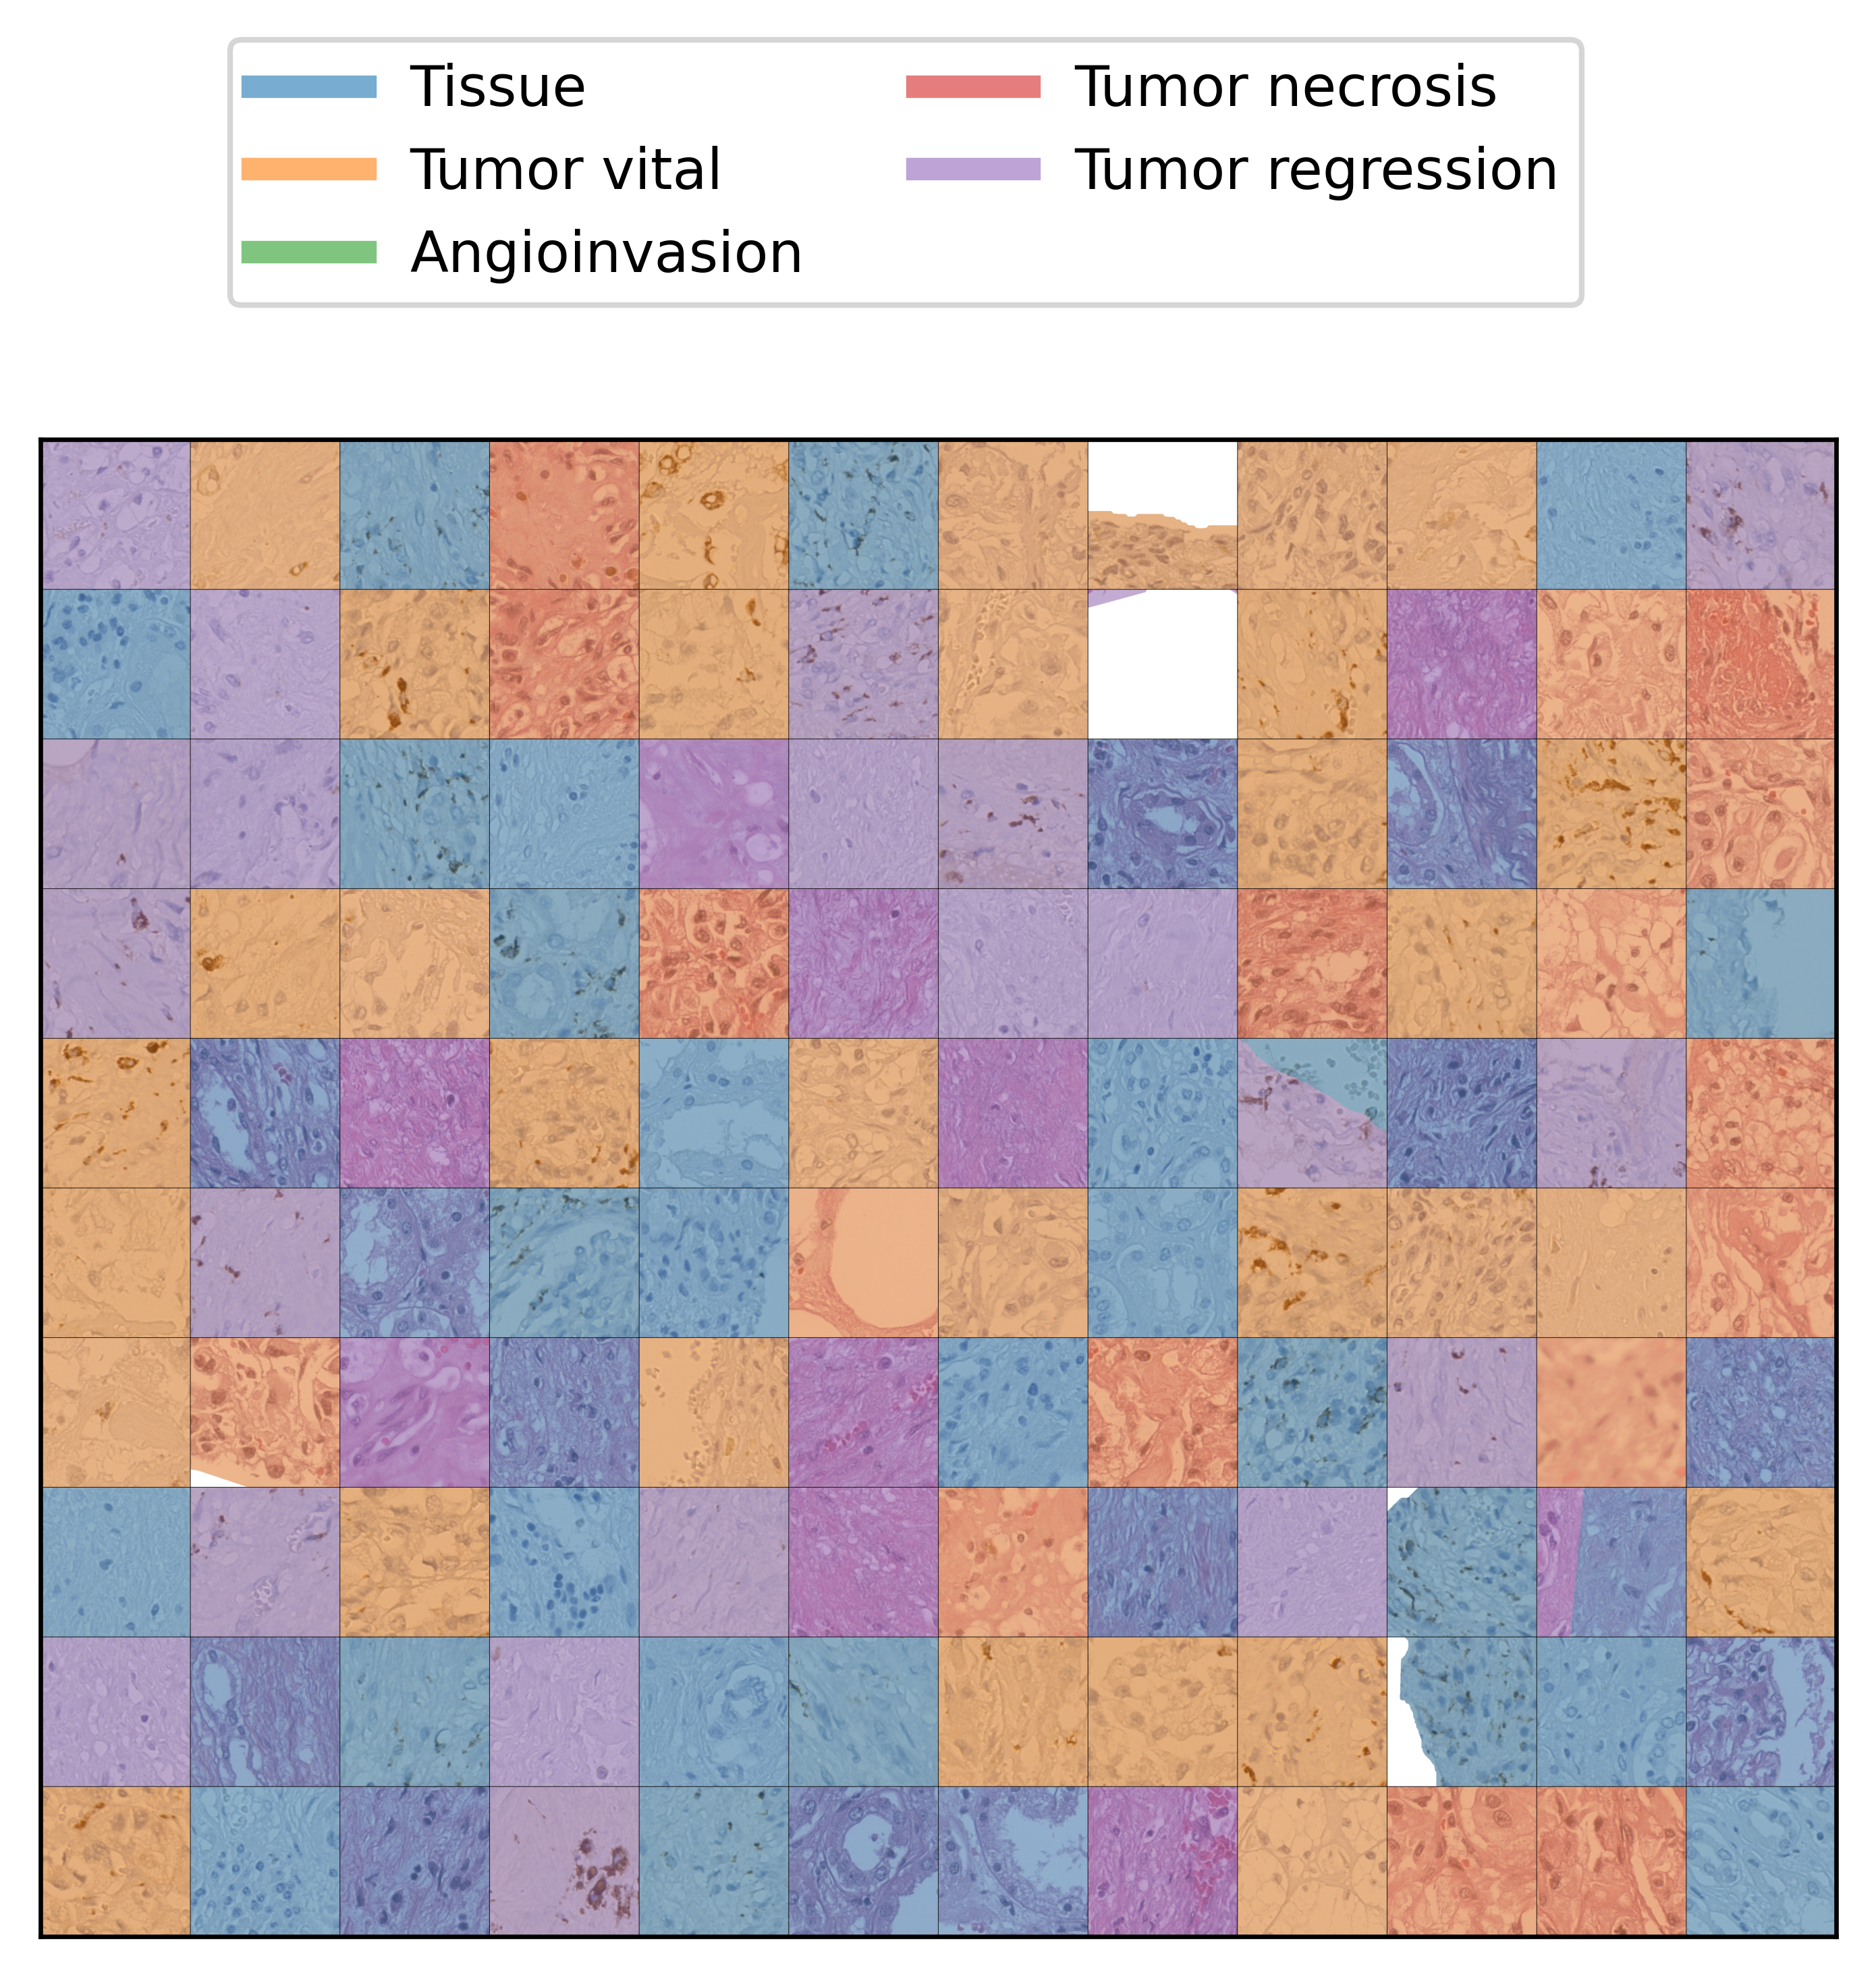
\includegraphics[width=0.75\textwidth]{latex/figures/postproc_subimage_1_(120, 12).png}
    \caption[Patch extraction]{Random selection of extracted patches with the corresponding mask overlaid in colour. White areas are not part of the tissue, but the empty background. Each patch has dimensions of 512x512 pixels and is extracted from a WSI with each dimension being at least close to 100,000 pixels.}
    \label{fig:patches}
\end{figure}

\subsection{Downsampled WSIs}
    \label{DownsampleData}
As mentioned above, an alternative approach to dividing images into patches is to load them at reduced resolution and size. Although fine-grained information is lost, this way, the spatial information can be maintained easily. Also, no bias is created, unlike random sampling of patches does. Moreover, this is computationally inexpensive, as each SVS file already contains versions of its image at lower resolutions. The general approach works as follows:

In a small preprocessing step, each tissue mask is loaded at the desired resolution to determine the respective maximum width and height of the tissue within the whole image. This is necessary because of the varying dimensions of each image. Also, due to quality issues of the scans, there are WSIs with a lot of whitespace. As a WSI scanner produces an WSI by scanning tiles on a grid, it usually skips tiles that do not contain tissue by checking an area of the glass slide at a higher resolution. The final output is then truncated to not contain large areas without tiles that were actually scanned. However, if such a tile contains contaminations such as dust, water droplets, etc. it will be scanned and the WSI cannot be truncated properly any more. Hence, the location of the tissue (top-right coordinate) to be used for later extraction of only relevant regions is stored as well. 
Fortunately, this pre-processing has to be done only once, since the representation of each sample can simply be stored according to JavaScript object notation (JSON). The created JSON file is an array of objects (a list of dictionaries in Python) where each object contains the paths to its SVS file and the corresponding masks in TIFF format. Furthermore, each record stores relevant metadata, such as the case ID, the stain code, the coordinate from where the tissue is to be extracted and the aforementioned maximum width and height over the entire data set. This has the advantage that the representation can be easily updated in \(O(k)\) where \(k\) is the number of new samples, rather than in \(O(n)\) where \(n\) represents the final size of the data set. Especially if the maxima remain the same, since existing records do not need to be updated at all. This approach allows to later load only the area of an image that actually contains tissue. Thus, it speeds up repetitive loading of images and masks during training without requiring significant amounts of extra storage. 

In the presented experiments, each WSI is read at level 3 which corresponds to a downsampling factor of 64. The images are padded equally on each side with zeroes until they equal the dimensions of the respective maxima determined earlier. There might be a shift towards the bottom or right by one pixel, which is the case if a completely even padding is not possible due to the respective dimensions of the image itself. This approach was chosen over simply resizing them to prevent a possible loss of information. Since all images are taken at the same magnification by the scanner, resizing them could distort the spatial information as objects get enlarged. Figure \ref{fig:downsample_input} visualises the input received by the neural network. The first three channels represent the image data in RGB format and are shown as a single image here. Stacked on top are the different masks in a pre-defined order.

\begin{figure}[h!t]
    \centering
    % \vspace{-14pt}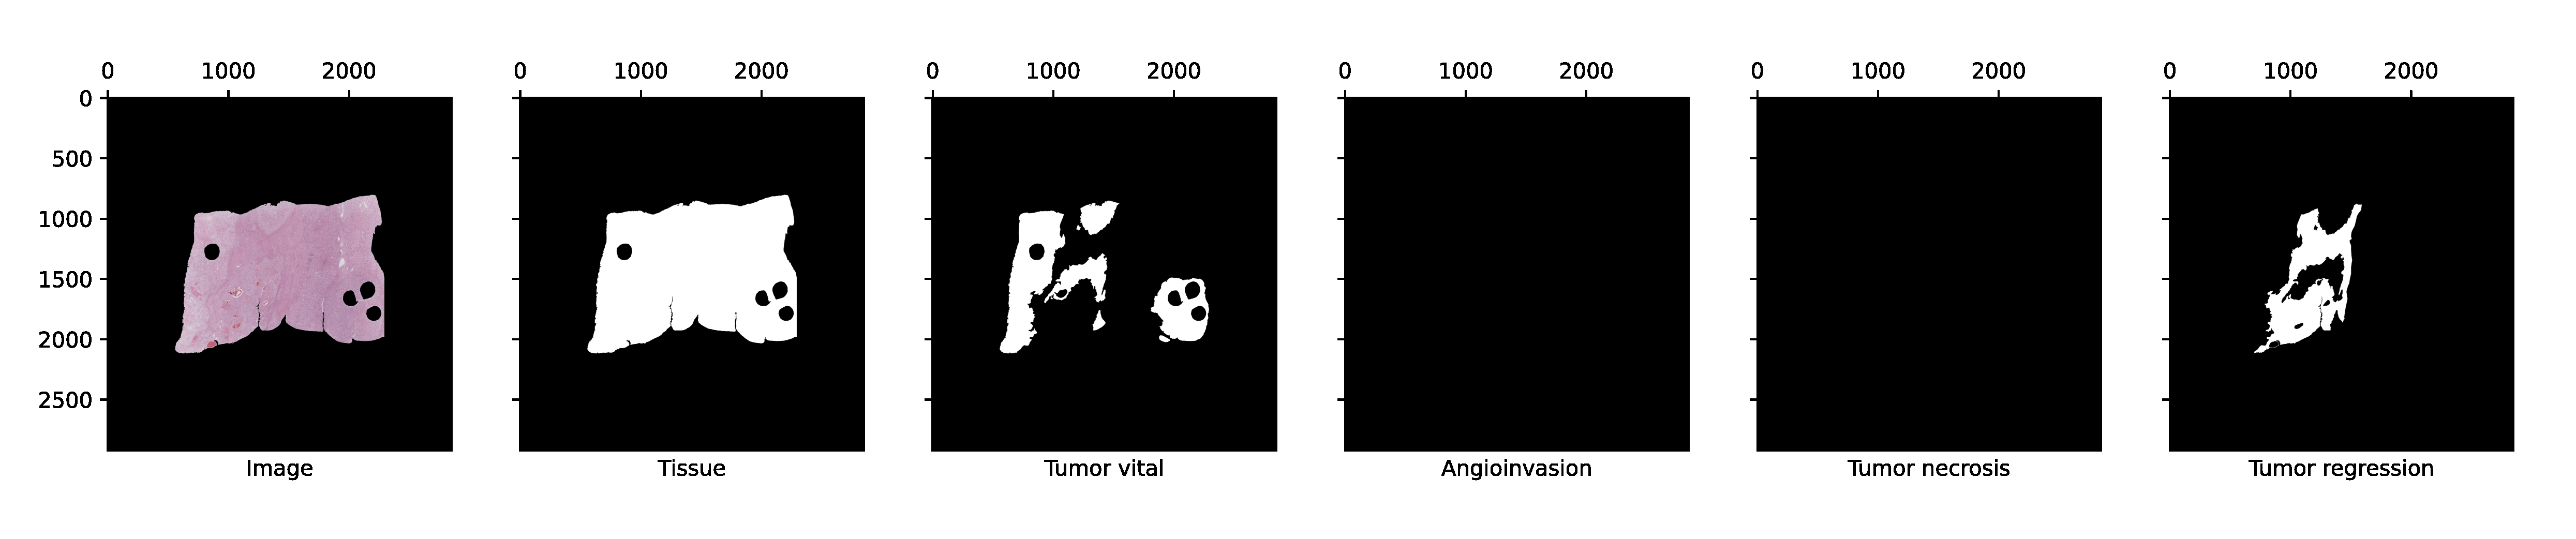
\includegraphics[width=\textwidth,trim={0 0 0 40pt},clip]{latex/tissue/AAA_postproc_subimage_1-1.png} \\
    \vspace{-14pt}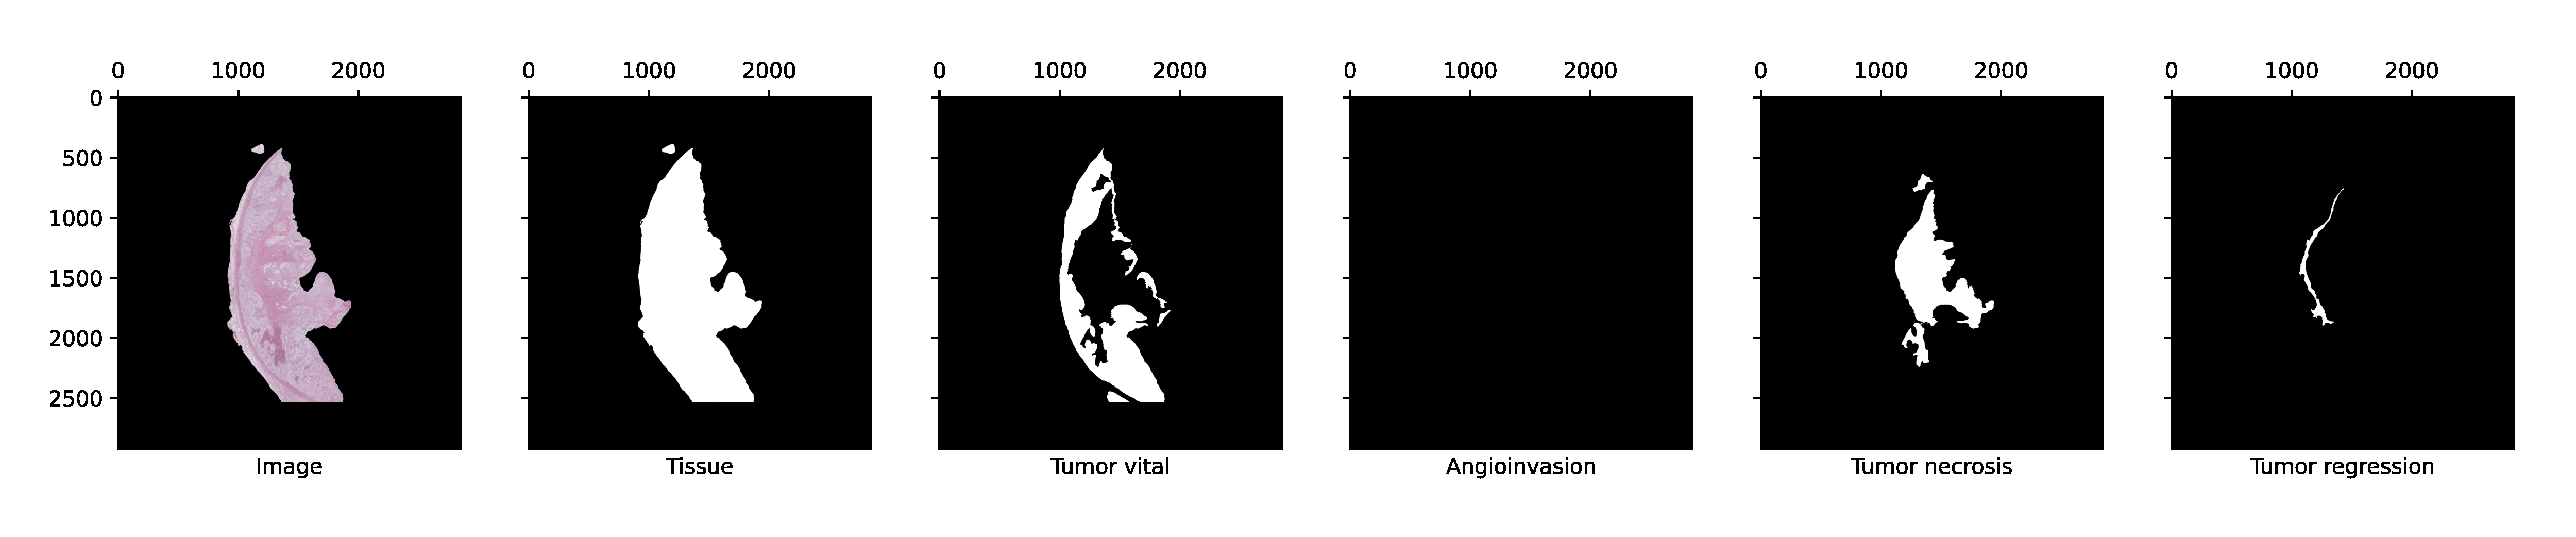
\includegraphics[width=\textwidth,trim={0 0 0 20pt},clip]{latex/tissue/AAA_postproc_subimage_3-1.png} \\
    \vspace{-14pt}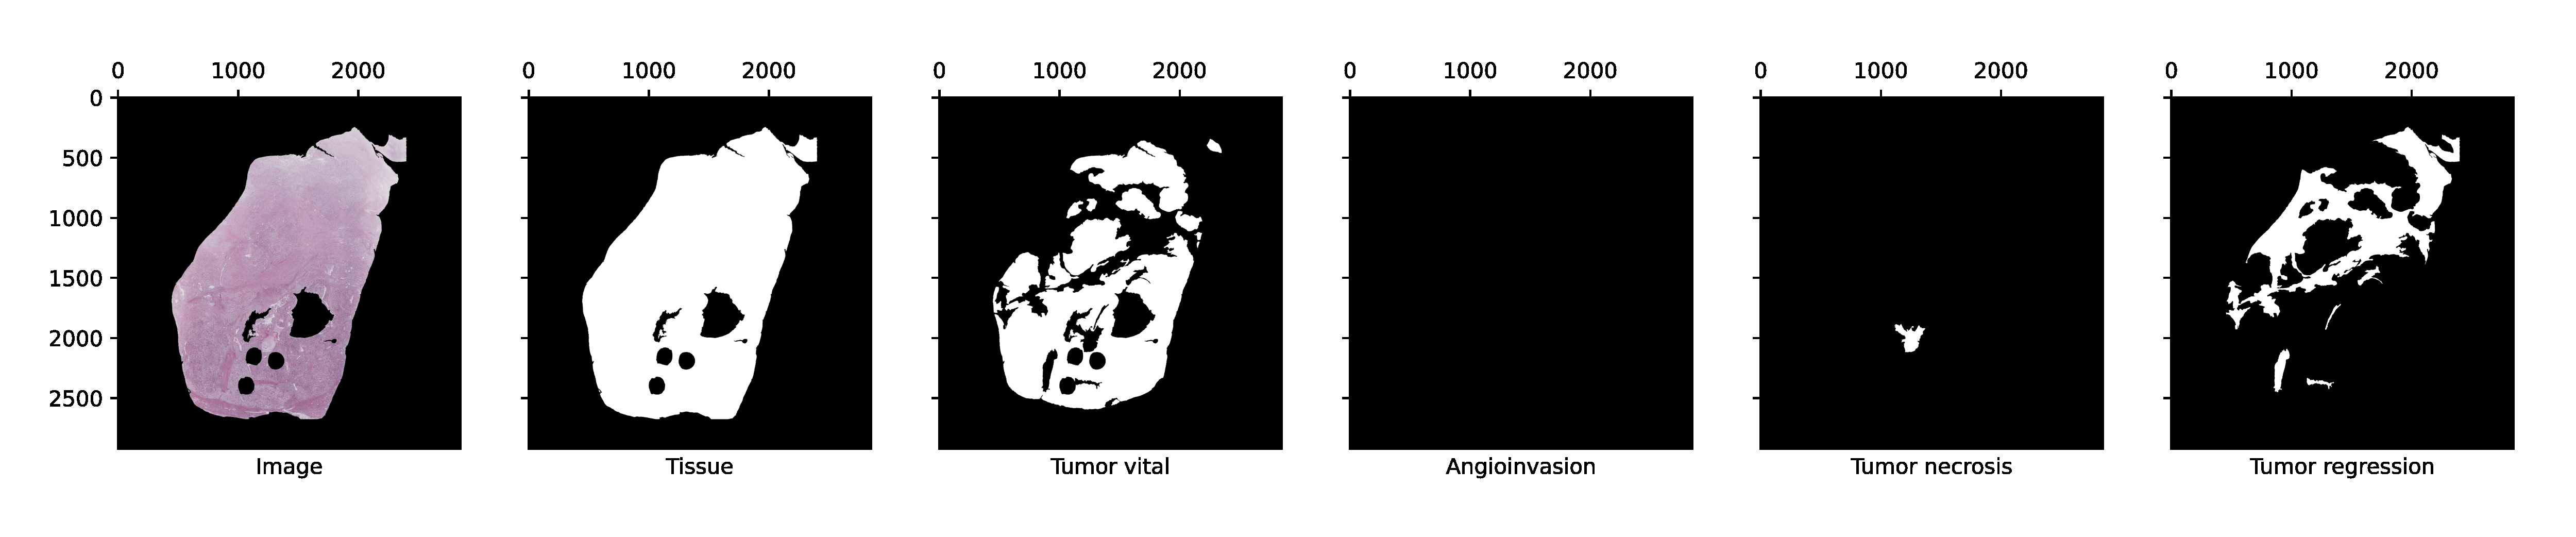
\includegraphics[width=\textwidth,trim={0 0 0 40pt},clip]{latex/tissue/AAA_postproc_subimage_12-1.png} \\ 
    \vspace{-14pt}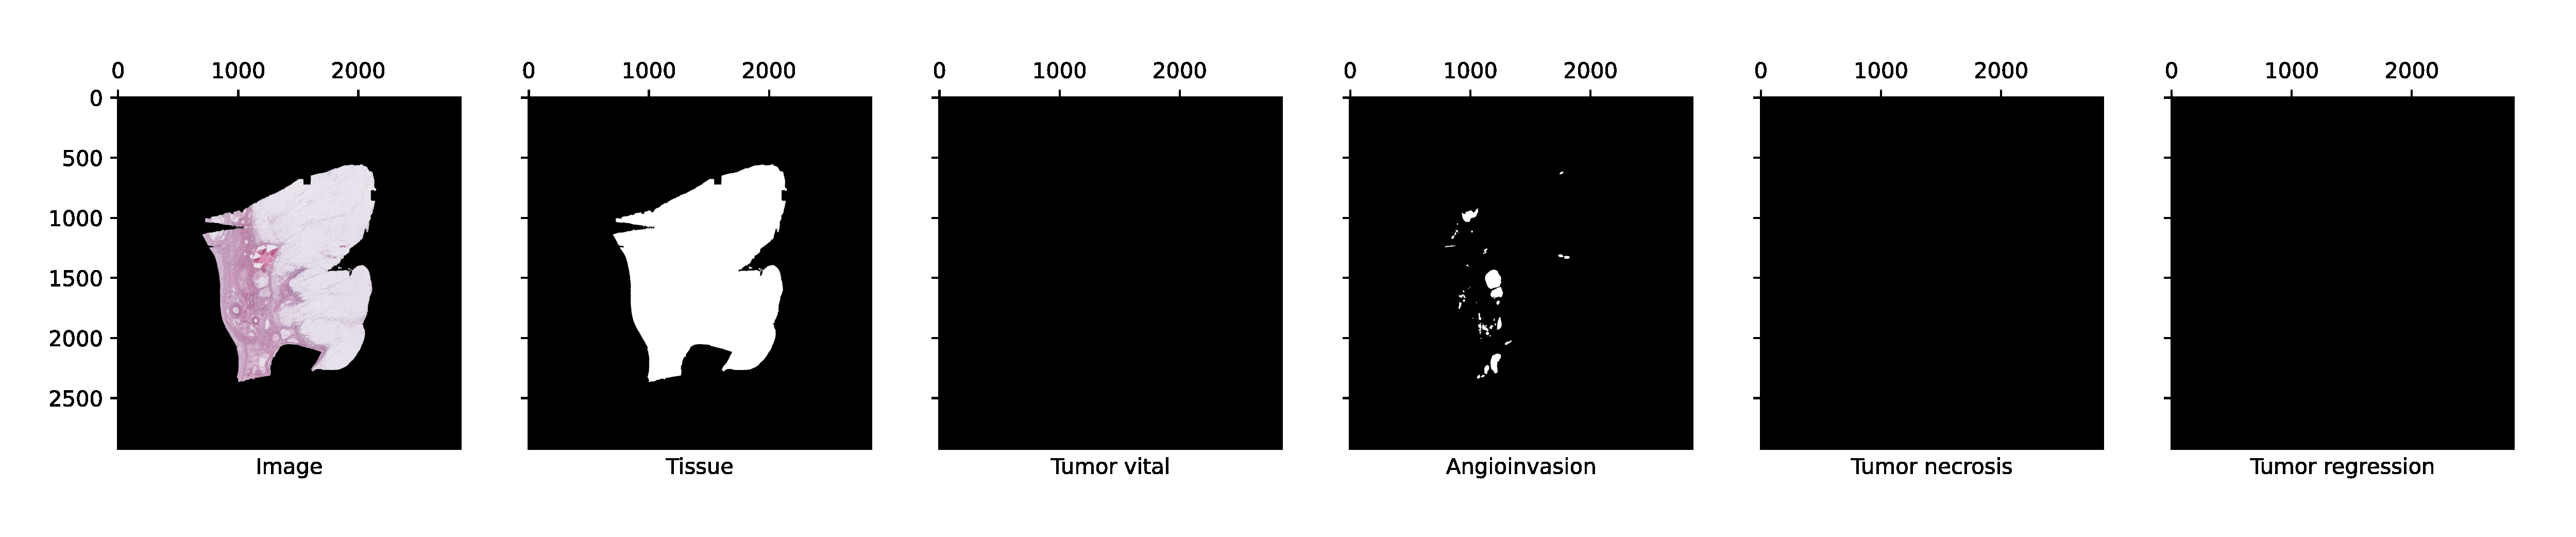
\includegraphics[width=\textwidth,trim={0 0 0 40pt},clip]{latex/tissue/AAA_postproc_subimage_19-1.png} \\
    \vspace{-14pt}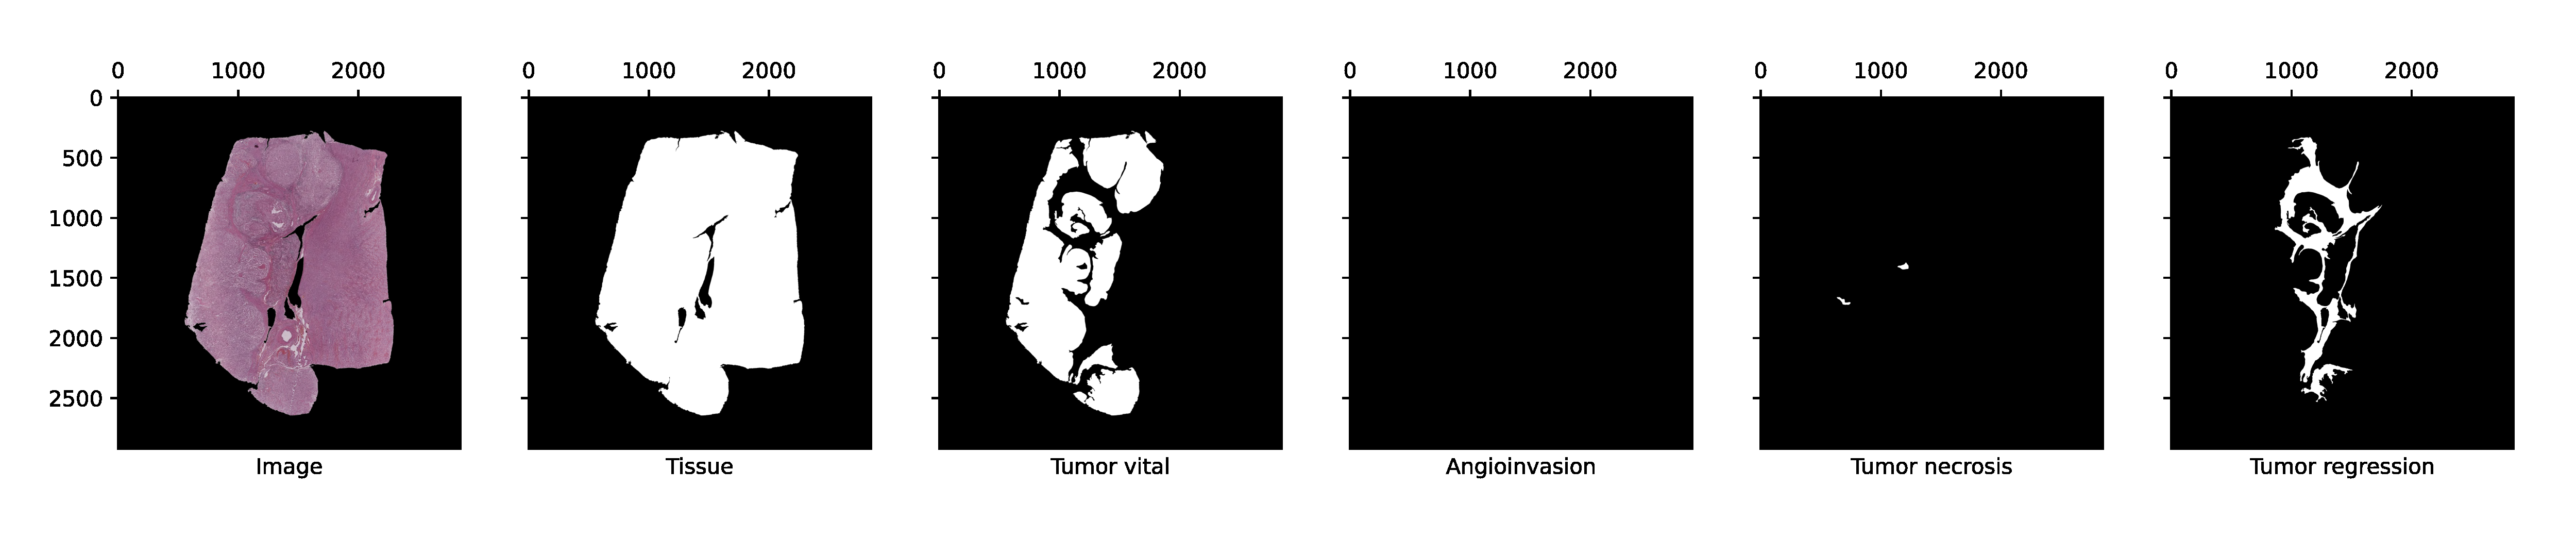
\includegraphics[width=\textwidth,trim={0 0 0 40pt},clip]{latex/tissue/AAA_postproc_subimage_158-1.png} \\
  \caption[Neural network input]{Representation of the input to the neural network. The “image” represents a tensor of dimensions CxHxW where C is 3. Each mask is a 2D tensor. All are stacked into a single 3D Tensor with 8 channel dimensions. Both axes represent the coordinates in pixels. Shown are the cases with IDs 1, 3, 12, 19 and 158 from top to bottom.}
  \label{fig:downsample_input}
\end{figure}

\subsection{Data Augmentation}

We use random transformations to augment the dataset and thus induce better generalization. For this purpose, the inputs are randomly flipped on both axes. This is applied to both the images themselves and the accompanying masks, independent of them being patches or downsampled slides. By this approach, we hope to prevent the network from overfitting on the shape of the objects presented. Especially since each patient contributes multiple samples that are similar in their high-level appearance, this is a possible risk.
Also, the WSIs brightness, contrast, and saturation are jittered by a small value. This is done to create minor variations between samples in addition to the larger ones already present. This helps to increase the generalization performance of the model, which is to be preferred over a higher score on the current dataset. The literature does support this approach, as it is common that scanners and stains do not produce not perfectly reproducible results. Hence, it makes sense to mimic this behaviour artificially. \cite{Macenko2009method, Ciompi2017importance}

\section{Network Architectures}
  \label{NetArch}

\subsection{WSI networks}

\subsubsection{ResNet} First, a ResNet-based CNN was used to analyse only all slides in a unimodal way. For this purpose, the implementation \verb | resnet101 | of the Python package \verb|torchvision| was chosen. The choice for a ResNet based architecture is rooted in the results of the chamelyon17 challenge, where this architecture was employed frequently with good results. \cite{Bandi2019Detection} Although, this challenge was carried out on a different task using different evaluation methods, we hypothesise that these findings are still applicable to our problem. Since CNN architectures are used as a means to extract features, i.e., to identify repeating higher-level structures in the image, the benefit to survival analysis can be expected to be similar.

However, these ResNet models expect an image in the RGB (Red-Green-Blue) colour space, i.e. the input is expected to be a 3-dimensional tensor with 3 channels in the outer dimension. Hence, a single convolutional layer was placed in front of the ResNet model to reduce the input dimensionality accordingly. This layer is accompanied by dropout and the rectified linear unit (ReLU) activation function, analogous to the original input layer of the ResNet architecture. 
These two conventional convolutional layers are followed by 4 residual blocks, each consisting of convolution, dropout, and batch norm layers followed by the ReLU activation function. The prediction of sample-specific risks was performed in two ways. First, by a single fully connected layer, thus transforming the 1000 input nodes into a single output value. In the second approach, the convolutional layers are followed by two fully connected (FC) layers. The first FC layer facilitates the learning of correlations between input to the hidden nodes. The second layer performs the prediction by outputting a single value. In the multimodal setting, the output of the first FC layer is fused with the other modalities and then processed by more FC layers. This potentially enables each modality to be first analysed separately and to look for within-modality interactions before considering cross-modality interactions as well. An illustration of these architectures can be found in the appendix \ref{fig:network_archs}. 
Due to memory requirements of our approach, only a batch size of 3 could be realised. This has the consequence that gradient accumulation was necessary to allow meaningful steps against the gradient. With this technique, multiple gradients are computed, and a step is taken on the average of these gradients only after a certain number of such iterations. Optimising over gradients that were computed with small amounts of samples increases the risk of inefficient steps which do not move the weights towards the minima of the true gradient of the full dataset. This is especially the case, if this small subset is not representative for the full dataset and can in turn slow down convergence significantly. Therefore, an initial accumulation factor of 12 was chosen, resulting in an effective batch size of 36. While a higher amount of accumulations might stabilise the training prices even further, it increasingly slows down training as well.
\subsubsection{EfficientNet} 
Besides ResNet, EfficientNetV2 was tested for image analysis of the WSIs. The \verb|torchvision| implementation \verb|efficientnet_v2_s| of EfficientNetV2 was used. Analogous to our ResNet approach, a preliminary convolutional block, modelled after the input layers of \verb|efficientnet_v2_s| reduces the number of channels of the input. 
The last convolutional layer of the model was replaced in order to be able to alter the size of the feature vector. A single linear layer was used for the prediction of hazards.
\subsubsection{Distributed Training} 
All training that involved the WSI data was carried out using the distributed data parallel paradigm, as implemented in the Python package \verb|PyTorch|. With this method, the dataset is divided among multiple GPUs and then processed in parallel. The weights and gradients are synchronised before and after each optimisation step. This allows us to increase the effective batch size by the number of GPUs deployed. Interestingly, the synchronisation overhead is reduced thanks to the accumulation of gradients that we perform. As synchronisation is only necessary during actual weight adjustments, the frequency of synchronisations is reduced. The more advanced paradigm Fully Sharded Data Parallel (FSDP) was also trialled, but no improvement in processing speed was observed. Meanwhile, the performance of the network itself remained identical under deterministic conditions. 
For actual training, the data was divided into splits of 75\%, 15\% and 5\% for training, validation and test sets, respectively. For the purpose of overfitting on 5\% of the data, a 50/50 split was performed between the training and validation set. This change was necessary, because the validation set would have contained too few uncensored samples otherwise. Hence, the subset of the data set consisted of 35 samples.
\subsubsection{Overfitting} 
Overfitting can be helpful in evaluating the capabilities of a model. It is desirable that a model is able to overfit on a small dataset, since that usually ensures that it contains sufficient complexity to represent the data. However, this must be regarded with some scepticism. Since the subset of data is chosen randomly, it is not guaranteed to represent the entire dataset or its complexity. This means that the model might not be able to overfit the full dataset but only the small subset of it, which defeats the purpose of these experiments. However, for the case of tissue slides, it is unlikely that some samples are drastically more or less complex than the other samples. For example, if we were to use a heterogenous dataset consisting of multiple cancer types or subtypes, this would be a more serious concern. 
Another issue are the binary masks, which are stacked on top of each WSI. Since only a few samples contain annotations for “Angioinvasion” or “Tumour Necrosis”, there is a high chance that WSIs with such annotations are not adequately represented. That is because these samples are scarce and their area is quite small if they are present. Therefore, the more concerning question would be whether something is learnt from these annotations at all.

\subsection{Processing Genomic Data}

Analogue to the WSI data, the gene count data from the NanoString assay was also analysed in isolation. For this, the Self normalizing network architecture previously employed by Chen et al. in PathomicFusion \cite{Chen2022Pathomic} was adapted. This network consists of four self-normalising layers. These types of layers were first proposed by Klambauer et al.\cite{Klambauer2017Self} Each layer consists of a fully connected layer, the scaled exponential linear unit (SeLU) as the activation function, and an Alpha dropout layer. These layers drive each output towards zero mean and unit variance; these properties are then maintained by Alpha Dropout. This strategy has been shown to prevent instabilities caused by vanishing or explosive gradients. \cite{Chen2022Pathomic}
These self normalising subnetwork is followed by a single fully connected layer that performs the prediction. In contrast to PathomicFusion, our network uses SeLU activation functions instead of Exponential Linear Units (ELU). For the purpose of training the neural network, each feature was standardised across samples using the \verb|StandardScaler| class from the Python package \verb|scikit-learn|. Figure \ref{fig:SNN} shows a visualisation of that network.

\begin{figure}[h!t]
    \centering
    \includegraphics[width=\textwidth]{latex/networks/genomic_snn.onnx_horz.png}
    \caption[Self Normalizing Network Diagram]{Self Normalizing network for NanoString Gene Expression data. The network consists of 4 blocks. Each is made up of a fully connected Layer (FC), Alpha Dropout (ADP) and a scaled exponential linear unit (SeLU). Lastly another fully connected layer performs the prediction. This figure was created using the Netron web tool. \cite{Roeder2023Netron}}
    \label{fig:SNN}
\end{figure}

\subsection{Fusion Network}

As our tests included some more involved methods, others are more straightforward. This section will explain each of them, starting with the strategies belonging to the latter category.

\subsubsection{Vector based fusion methods} 
These methods all consist of simple vector operations. For once, we take the element-wise sum of the feature vectors, hence using a single vector of the same size as the unimodal ones as input to the network. In the same manner, the element-wise product and the element-wise maximum of features are tested as well. However, by concatenating the unimodal feature representations, the last of these simple approaches does change the shape of the input to the prediction network. We deal with the doubled length by adjusting the input size of the following fully connected layer accordingly.

\subsubsection{EmbraceNet} The EmbraceNet \cite{Choi2019EmbraceNet} approach was already briefly mentioned in chapter \ref{related}. We apply only the fusion part of EmbraceNet, i.e. the embracement layers as a fusion technique. We do not require the use of docking layers, as we train the subnetworks of our end-to-end model to learn feature representations of the same dimensionality. This fusion approach is based on probabilities, where each position of the input vectors is assigned a probability that decides from which input vectors the respective value should be taken. If a modality is missing, their probabilities are set to zero. For our bimodal approach, that means that the input is treated as unimodal for cases where the genomic data is missing. Despite that, all modalities present have equal probabilities of being picked for an element of the output vector otherwise.

\subsubsection{Kronecker-based fusion} For this approach, we adopted the PathomicFusion methodology proposed by Chen et al. Our implementation is very closely modelled after their bimodal fusion method. In this approach, the learnt feature representations are fused by computing the Kronecker product, which is the outer product between all the unimodal vectors. For the bimodal approach, this means that the input are two 1D vectors of the same size, one for the WSI data and the other for the genomic data. The output then is a 2D matrix with dimensions equal to the length of each vector. However, there is a preliminary step that aims to improve the results. In order to reduce the impact of noisy unimodal features, a gating-based attention mechanism is placed between the unimodal networks and the fusion mechanism. With this mechanism, we learn the importance of each feature in each unimodal vector with respect to the other modalities. The softmax probabilities of the resulting attention weights are applied to each unimodal representation. Afterwards, the vectors are fused as described above. \cite{Chen2022Pathomic} Due to the size of our feature vectors, we had to downsample using bilinear transformations.  Hence, a four times smaller representation had to be created before Kronecker fusion could be applied.   

\subsubsection{Attention} This approach employs a simple attention layer to produce attention weights for each unimodal feature vector. This is done with a single fully connected layer where the input size is equal to the output size, and no bias term is used. This layer is combined with the hyperbolic tangent activation function, followed by a softmax operation. During backpropagation, the weights of this layer are trained to be directly interpretable as feature importance weights. Each attention vector is then applied to its respective feature vector by element-wise multiplication. Afterwards, the sum of the attended feature vectors is taken in order to receive a 1D input for prediction. However, in this approach, missing modalities are factored in by scaling up the values of the fused vector, where the values are multiplied by the count of empty modalities.

\section{Experimental exploration}

% \subsection{Hardware}

The unimodal SNNs were trained on a single NVIDIA GeForce RTX 3060 Ti GPU. Both the unimodal WSI networks and the fusion networks were trained on 4 NVIDIA A40 GPUs using Distributed Data Parallel and \verb|pytorch|. Before we could train the network with the settings as described in chapter \ref{Results}, various tests were necessary. For once, we tried to train the image network with WSI at the larger levels (4x, 16x) first, only to find that that was not feasible. Furthermore, multiple different approaches for efficient handling of the data were explored as well. 

A copy of the code is available at the department of Data Science in Biomedicine at the Peter L. Reichertz Institute for Medical Informatics (PLRI) and an updated version will also be publicly be available in the foreseeable future at \url{github.com/seapat/renal-cancer-dl}.


% The first attempt was to train on a downsampled resolution. This was a seemingly easy approach, since, thanks to the pyramidal tiff files, images at lower resolutions were already available. That being said, there are many issues with this Approach, all stemming from memory limitations. Firstly, loading images at the first downsampling resolution (4x) was not possible, as a single sample did not fit into memory. 
% At the second level (16x), a mini-batch with a size of two is possible. However, this causes problems for a considerable subset of samples. Since the loss ignores censored samples, there is a risk that both samples are censored, and a sensual negative log-likelihood cannot be computed. Gradient accumulation helps with this

% \subsection{Nanostring data}

% We run comparisons to determine the impact of different hyperparameters by modifying a single one while leaving all other hyperparameters fixed. We chose to first adjust the learning rate to find the most promising one. From that starting point, we compared different dropout probabilities and different lengths for the feature vector that serves as input either to the prediction in the unimodal case, or for the  multimodal fusion. For the first comparison, the same dropout  rate was applied to all layers. We tested values 0.1, 0.25 and 0.5. For the second comparison, four different sizes were evaluated. Namely, vectors of length 250, 500, 750 and 1000 were returned. 

% \section{Interpretability Methods}

% All employed methods for model interpretability were implemented using the Python packages \verb|captum|. The Saliency, Input X Gradient, Integrated Gradients and GradCAM algorithms were used to gain insights on the feature attribution of the image data. For this purpose, the best-performing unimodal model trained on the WSI data was used. For each method, the 
% %TODO: specify outlier_perc, ie number of extremes that were ignored.